\documentclass[tikz]{standalone}
\usepackage{tikz}
\usetikzlibrary{patterns,snakes, angles}
 
\begin{document}
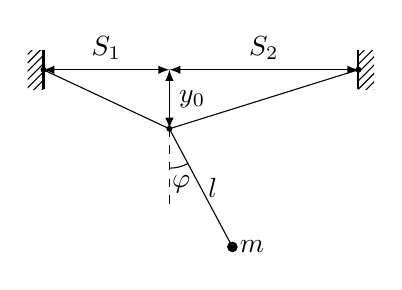
\begin{tikzpicture}
	\draw [draw=none, pattern=north east lines] (0,0) rectangle (-0.2,0.5);
	\draw [thick] (0,0) -- (0,0.5);
	\draw [draw=none, pattern=north east lines] (4,0) rectangle (4.2,0.5);
	\draw [thick] (4,0) -- (4,0.5);
	\draw [fill] (0,0.25) circle (0.03);
	\draw [fill] (4,0.25) circle (0.03);
	\draw [fill] (1.6,-0.5) circle (0.03);
	\draw [arrows={latex-latex}] (0,0.25) -- (1.6,0.25) node [midway, above] {$S_1$};
	\draw [arrows={latex-latex}] (1.6,0.25) -- (4,0.25) node [midway, above] {$S_2$};
	\draw (0,0.25)--(1.6,-0.5)--(4,0.25);
	\draw (1.6,-0.5) -- (2.4,-2);
	\draw [fill] (2.4,-2) circle (0.06);
	\node at (2.15,-1.25) {$l$};
	\node at (2.65, -2) {$m$};
	\draw [arrows={latex-latex}] (1.6,0.25) -- (1.6,-0.5) node [midway, right] {$y_0$};
	\draw [dashed] (1.6,-0.5) -- (1.6,-1.5);
	\coordinate (A) at (1.6,-1);
	\coordinate (B) at (1.6,-0.5);
	\coordinate (C) at (2.4,-2);
	\pic [draw, -, angle eccentricity=1.5] {angle = A--B--C};
	\node at (1.75,-1.2) {$\varphi$};
	
\end{tikzpicture}
\end{document}